\section{Experiments}
\label{sec:experiments}
We use all the environments  introduced in \citet{plappert2018multi} for our experiments.
Broadly the environments fall in two categories, Fetch tasks and Hand tasks.

The Fetch task involves a 7-DOF robotic arm. The four tasks are Reach, Push,
Slide and PickAndPlace.
In the Reach task the arm's end-effector is to reach the a particular 3D coordinate. 
In the Push task a block on a table needs to be pushed to a given point on it.
In the Slide task a puck must be slid to a desired location.
In the Pick And Place task a block on a table must be picked up and moved to a
3D coordinate.

The Hand tasks uses simulation of Shadow dexterous hand to manipulate objects of
different shapes and sizes. These tasks include HandReach,
HandManipulateBlockRotateXYZ, HandManipulateEggFull and HandManipulatePenRotate.
The HandReach task needs the finger tips to reach a given configuration.
In the HandManipulateBlockRotateXYZ, the a cubic block needs to be rotated to a
desired orientation in the Hand.
For HandManipulateEggFull an eggs needs to be moved and rotated to a given
position and orientation.
To complete the HandManipulatePenRotate task an pen needs to be rotated to a
certain goal orientation.

Snapshots of all these tasks can be found in Figure~\ref{fig:envs}. Note that
these tasks do not take visual input, but only joint angles from the arm and the hand.


\subsection{Metrics}
Similar to prior work, we evaluate all experiments on two metrics: the success
rate and the average distance to the goal. The success rate is defined as the
fraction of episodes in which the agent is able to reach the goal within a
pre-defined threshold region.
% $\frac{1}{E}\sum_{e,t} \mathbbm{1}_{\|\goal_t - \goal^*\|_2 < \epsilon}$.
The distance of the goal is euclidean distance of the
achieved goal from the desired goal.
% $\|\goal_t - \goal^*\|_2$.
These metrics are plotted against the number of training epochs showing
comparable results of our method to the baselines.

To emphasize that our method does not require goal-reward
and reward re-computation, we plot these metrics against
number of reward computations used during training.

%
\begin{figure}%
  \def\frac{0.24}
  \rotatebox{90}{\hspace{2em}\color{blue}{\tiny Fetch Reach}}%
  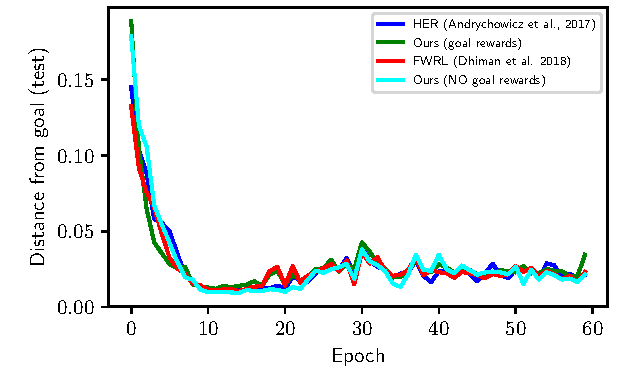
\includegraphics[width=\frac\columnwidth]{media/res/6efc1de-path_reward_low_thresh_chosen-FetchReachPR-v1-dqst/epoch-test/ag_g_dist.pdf}%
  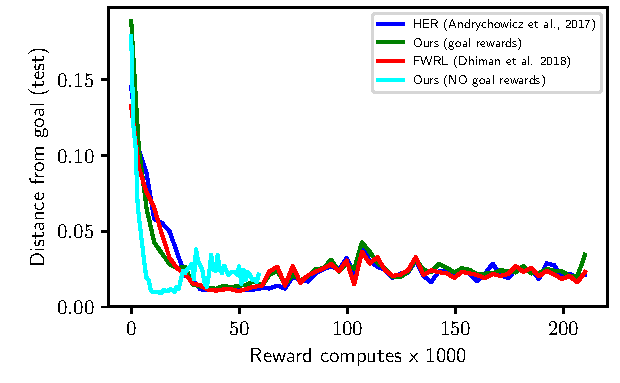
\includegraphics[width=\frac\columnwidth]{media/res/6efc1de-path_reward_low_thresh_chosen-FetchReachPR-v1-dqst/reward_computes-test/ag_g_dist.pdf}%
  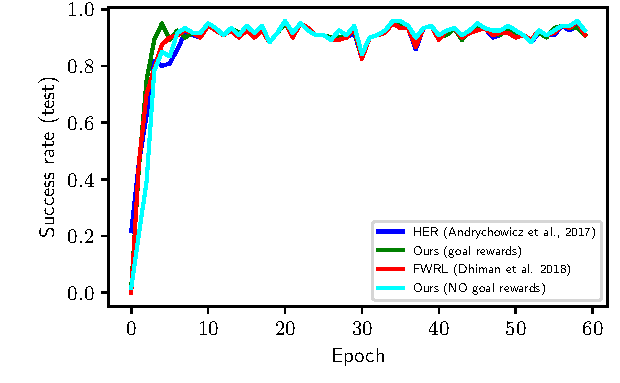
\includegraphics[width=\frac\columnwidth]{media/res/6efc1de-path_reward_low_thresh_chosen-FetchReachPR-v1-dqst/epoch-test/success_rate.pdf}%
  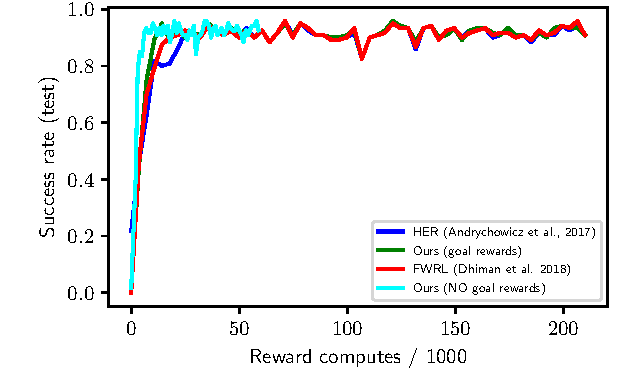
\includegraphics[width=\frac\columnwidth]{media/res/6efc1de-path_reward_low_thresh_chosen-FetchReachPR-v1-dqst/reward_computes-test/success_rate.pdf}\\
  \rotatebox{90}{\hspace{2em}\color{blue}{\tiny Fetch Push}}%
  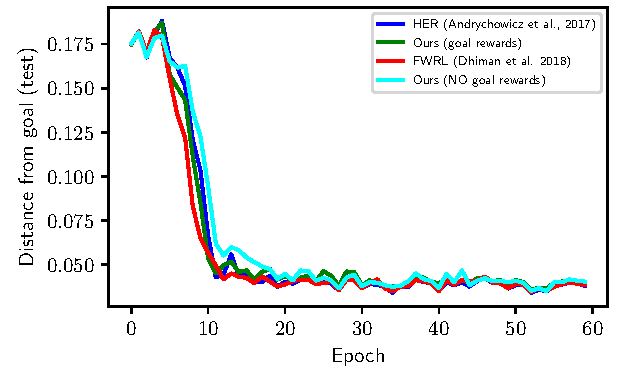
\includegraphics[width=\frac\columnwidth]{media/res/6efc1de-path_reward_low_thresh_chosen-FetchPushPR-v1-dqst/epoch-test/ag_g_dist.pdf}%
  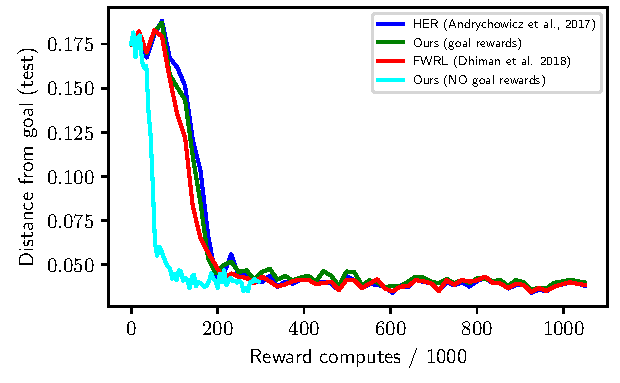
\includegraphics[width=\frac\columnwidth]{media/res/6efc1de-path_reward_low_thresh_chosen-FetchPushPR-v1-dqst/reward_computes-test/ag_g_dist.pdf}%
  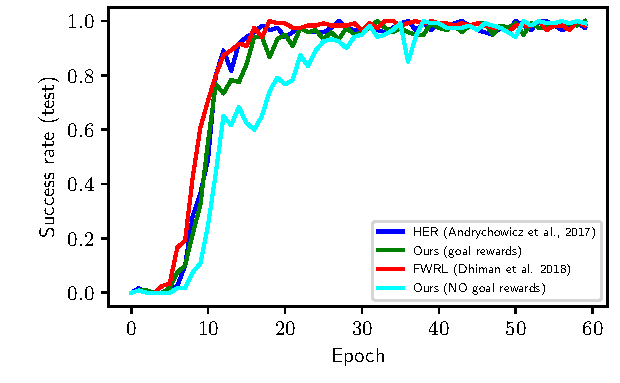
\includegraphics[width=\frac\columnwidth]{media/res/6efc1de-path_reward_low_thresh_chosen-FetchPushPR-v1-dqst/epoch-test/success_rate.pdf}%
  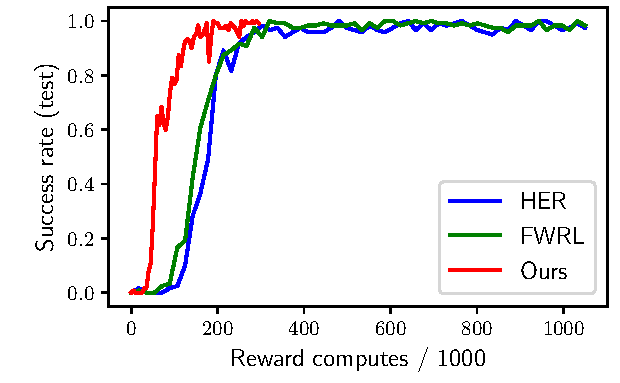
\includegraphics[width=\frac\columnwidth]{media/res/6efc1de-path_reward_low_thresh_chosen-FetchPushPR-v1-dqst/reward_computes-test/success_rate.pdf}\\
  \rotatebox{90}{{\tiny\hspace{1em} \color{blue}{Fetch Pick And Place}}}%
  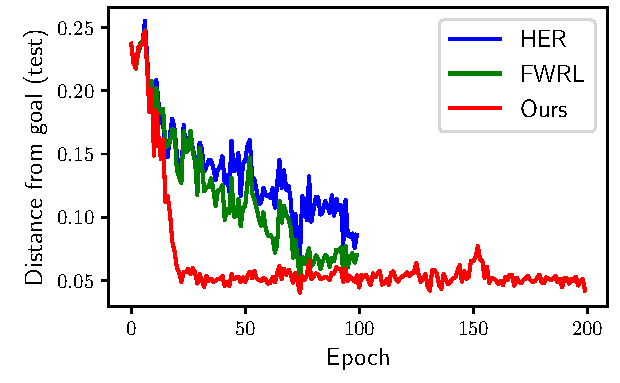
\includegraphics[width=\frac\columnwidth]{media/res/6efc1de-path_reward_low_thresh_chosen-FetchPickAndPlacePR-v1-dqst/epoch-test/ag_g_dist.pdf}
  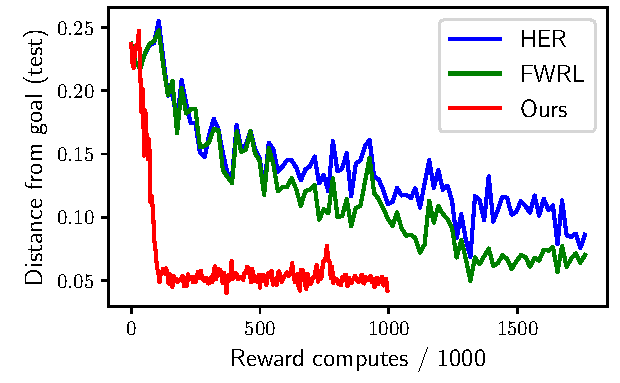
\includegraphics[width=\frac\columnwidth]{media/res/6efc1de-path_reward_low_thresh_chosen-FetchPickAndPlacePR-v1-dqst/reward_computes-test/ag_g_dist.pdf}%
  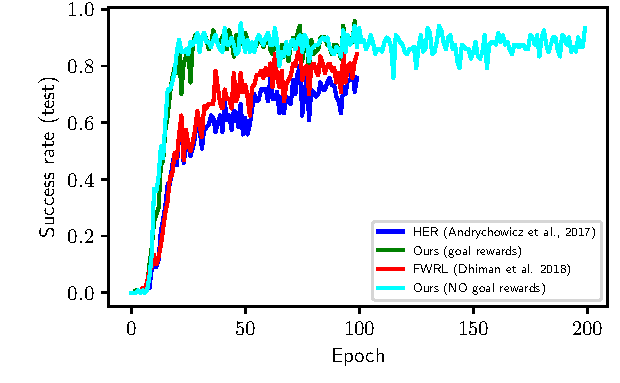
\includegraphics[width=\frac\columnwidth]{media/res/6efc1de-path_reward_low_thresh_chosen-FetchPickAndPlacePR-v1-dqst/epoch-test/success_rate.pdf}%
  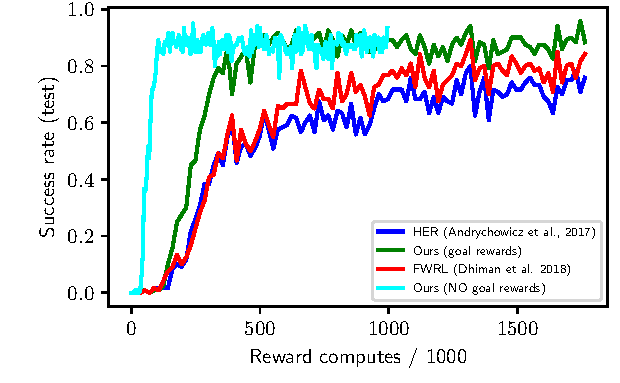
\includegraphics[width=\frac\columnwidth]{media/res/6efc1de-path_reward_low_thresh_chosen-FetchPickAndPlacePR-v1-dqst/reward_computes-test/success_rate.pdf}\\
  \rotatebox{90}{\tiny\hspace{2em}\color{blue}{Fetch Slide}}%
  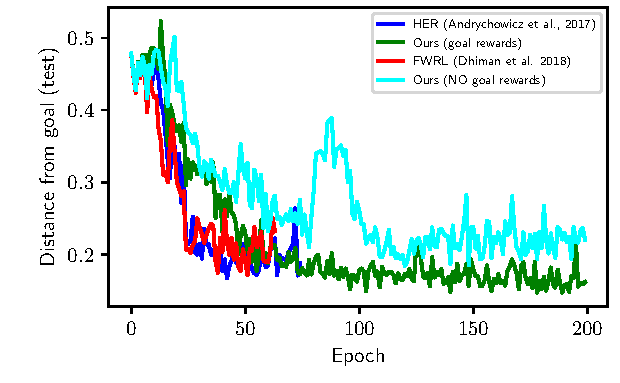
\includegraphics[width=\frac\columnwidth]{media/res/6efc1de-path_reward_low_thresh_chosen-FetchSlidePR-v1-dqst/epoch-test/ag_g_dist.pdf}
  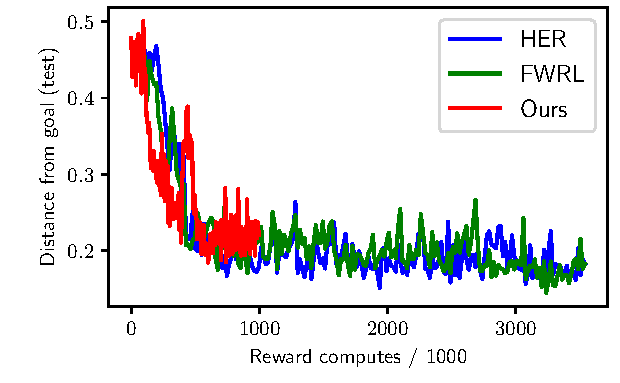
\includegraphics[width=\frac\columnwidth]{media/res/6efc1de-path_reward_low_thresh_chosen-FetchSlidePR-v1-dqst/reward_computes-test/ag_g_dist.pdf}%
  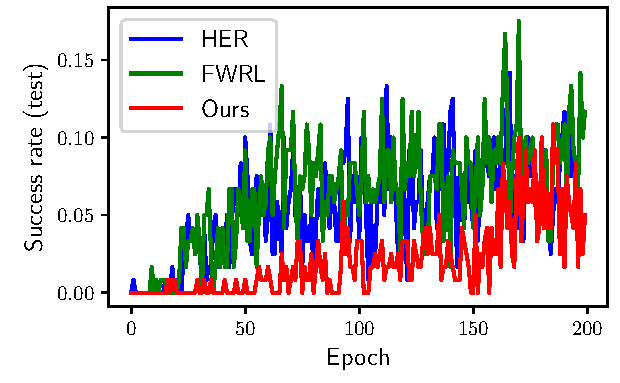
\includegraphics[width=\frac\columnwidth]{media/res/6efc1de-path_reward_low_thresh_chosen-FetchSlidePR-v1-dqst/epoch-test/success_rate.pdf}%
  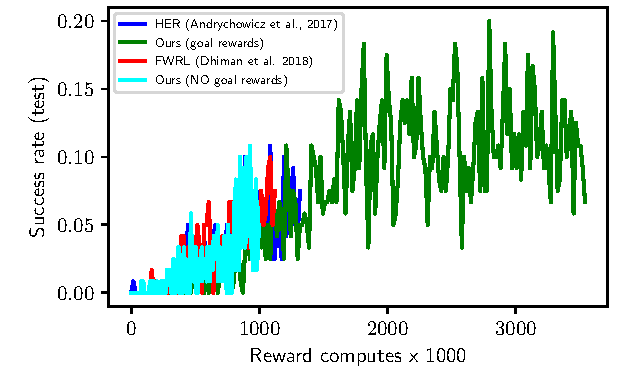
\includegraphics[width=\frac\columnwidth]{media/res/6efc1de-path_reward_low_thresh_chosen-FetchSlidePR-v1-dqst/reward_computes-test/success_rate.pdf}\\
  {.\tiny\color{blue}\hspace{0.8cm}(a) Distance on Epochs \hspace{1.05cm}(b) Distance on
    reward computes
    \hspace{0.70cm} (c) Success rate on epochs \hspace{0.9cm} (d) Success rate on reward computes}
    \caption{For the fetch tasks, we compare our method (red) against HER (blue) ~\citep{andrychowicz2016learning}
    and FWRL (green) ~\citep{dhiman2018floydwarshall} for the distance-from-goal
    and success rate metrics. Furthermore both metrics are plotted
    against two progress measures, the number of training epochs and the number of reward
    computations. Except for the Fetch Slide task, we get comparable or
    better performance across the metrics and progress measures. 
    }%
  \label{fig:fetch-results}%
\end{figure}


\subsection{Hyper-parameters choices}
Unless specified all our hyper-parameters are identical to the used HER
implementation~\citep{dhariwal2017baselines}. We note two main changes
to HER to make the comparison more fair. Firstly,
we use a smaller distance threshold.
The environment used for HER and FWRL returns the goal-reward when the
achieved goal is within distance threshold of the desired goal. In the absence
of goal-rewards the distance threshold information is not used by our
method.
We reduce the distance threshold to 1cm which
is reduction by a factor of 5.

Secondly, due to hardware limitations we run all experiments on six
cores each
while HER uses 19, which causes smaller batches to be used compared to the
published results. This may in turn lead to differences in the HER results.

However, all experiments are run with the same hyper-parameters and
random seeds to ensure that all variations in performance are purely due
to differences between the algorithms.

\subsection{Results}
% Due to space limitations and in the interest of clarity we show a subset our experiments across both platforms that emphasize both strengths and weaknesses of our algorithm.
All our experimental results are described below. We highlight the strengths and
weaknesses of our algorithm.

\subsubsection{Fetch Tasks}

For Fetch Reach and Push tasks our method achieves comparable performance
across both metrics, the success rate and the distance to the goal. In the Fetch
Pick and Place task, our method outperforms the baselines. However, for Fetch
Slide task the opposite is true.
When the number of reward computations is take into account our method learns
much faster than across all tasks.

\subsubsection{Hand Tasks}

For the Hand tasks the distance to the goal and the success rate show different trends.

For the distance metric when plotted against epochs, we get comparable
performance for all tasks; when plotted for reward computations we outperform
all baselines.

Similar trends does not hold for the success rate and we find our method to be
consistently under-performing than the baselines across all tasks. We note that
although all algorithms are equally far away from the goal, the success rate of
baselines is better than our method. We conjecture that this might be because of
high distance failure cases of the baselines. The baselines success rate is
high, but when they fail, they fail with a larger distance to the goal. This is
in contrast to our method which fails consistently but with still ends up closer
to the goal. On an average all methods end up showing similar distance from the goal.

\begin{figure}
  \def\frac{0.24}
  \rotatebox{90}{{\tiny \hspace{0.5cm} \color{blue}{Hand Reach}}}%
  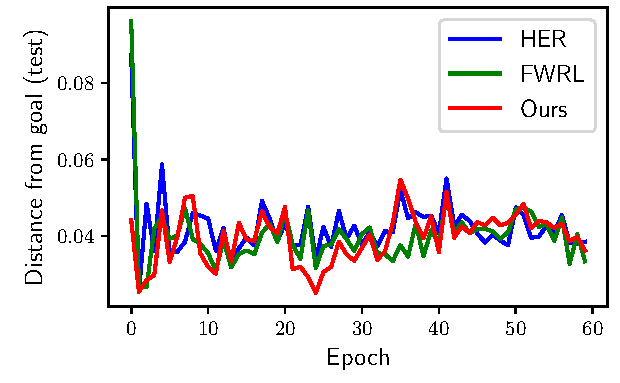
\includegraphics[width=\frac\columnwidth]{media/res/6efc1de-path_reward_low_thresh_chosen-HandReachPR-v0-dqst/epoch-test/ag_g_dist.pdf}%
  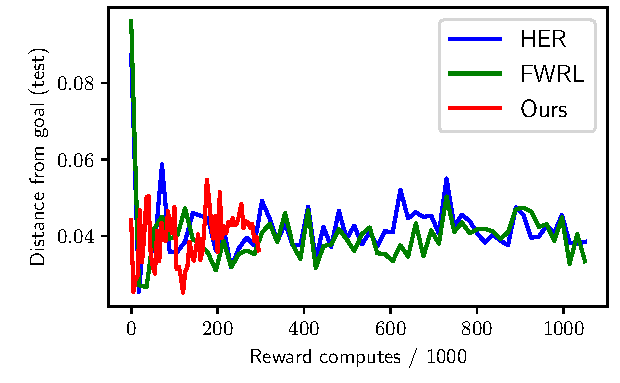
\includegraphics[width=\frac\columnwidth]{media/res/6efc1de-path_reward_low_thresh_chosen-HandReachPR-v0-dqst/reward_computes-test/ag_g_dist.pdf}%
  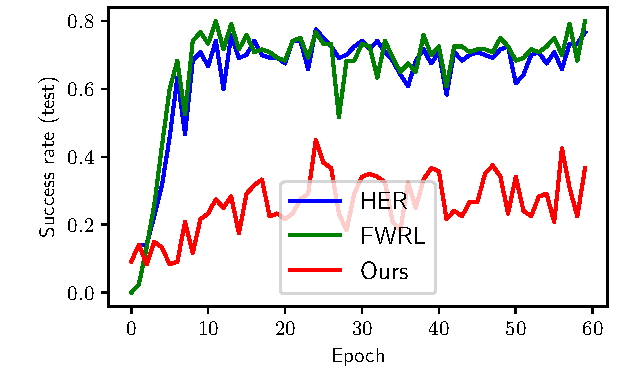
\includegraphics[width=\frac\columnwidth]{media/res/6efc1de-path_reward_low_thresh_chosen-HandReachPR-v0-dqst/epoch-test/success_rate.pdf}%
  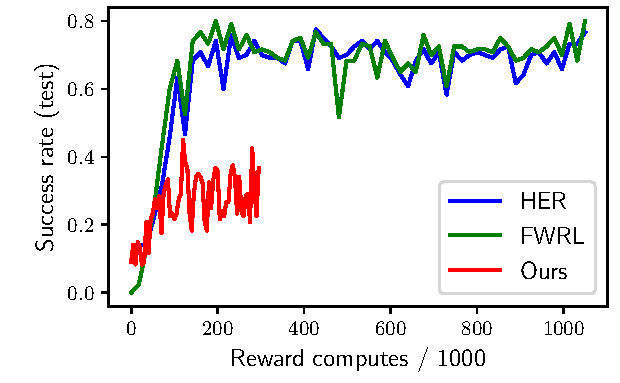
\includegraphics[width=\frac\columnwidth]{media/res/6efc1de-path_reward_low_thresh_chosen-HandReachPR-v0-dqst/reward_computes-test/success_rate.pdf}\\
  \rotatebox{90}{{\tiny \hspace{1em} \color{blue}{Hand Block Rotate}}}%
  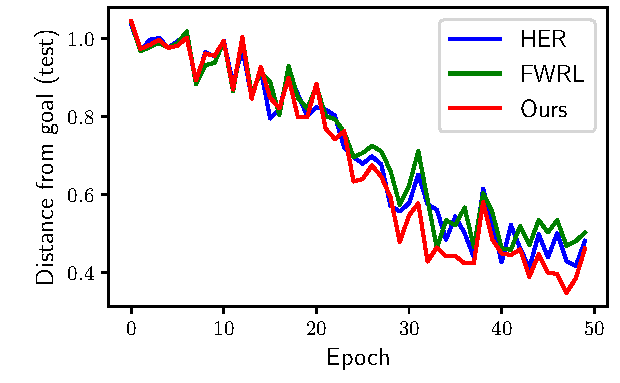
\includegraphics[width=\frac\columnwidth]{media/res/6efc1de-path_reward_low_thresh_chosen-HandManipulateBlockRotateXYZPR-v0-dqst/epoch-test/ag_g_dist.pdf}%
  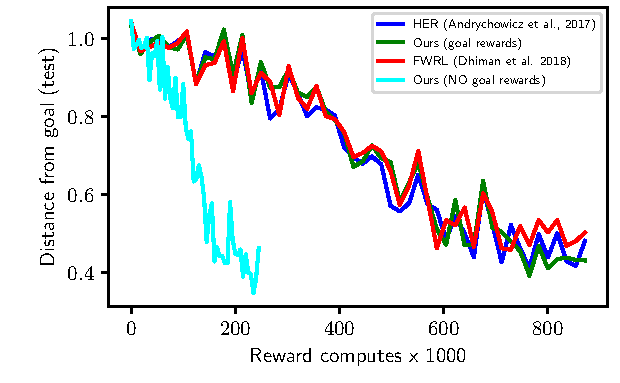
\includegraphics[width=\frac\columnwidth]{media/res/6efc1de-path_reward_low_thresh_chosen-HandManipulateBlockRotateXYZPR-v0-dqst/reward_computes-test/ag_g_dist.pdf}%
  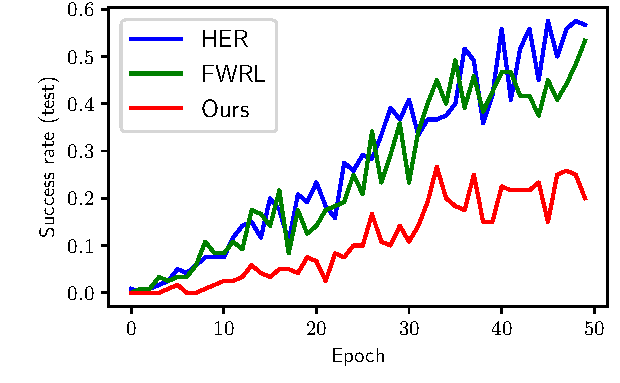
\includegraphics[width=\frac\columnwidth]{media/res/6efc1de-path_reward_low_thresh_chosen-HandManipulateBlockRotateXYZPR-v0-dqst/epoch-test/success_rate.pdf}%
  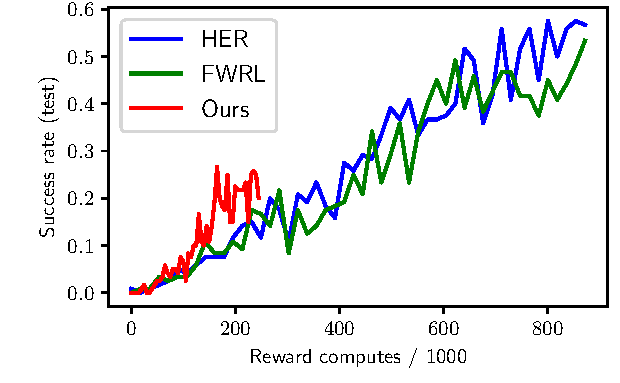
\includegraphics[width=\frac\columnwidth]{media/res/6efc1de-path_reward_low_thresh_chosen-HandManipulateBlockRotateXYZPR-v0-dqst/reward_computes-test/success_rate.pdf}\\
  \rotatebox{90}{{\tiny \hspace{0.7cm} \color{blue}{Hand Egg}}}%
  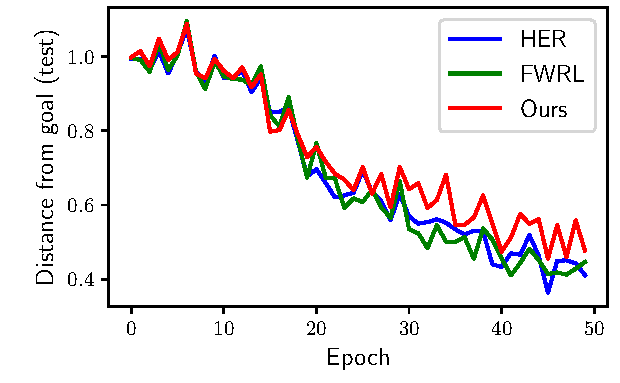
\includegraphics[width=\frac\columnwidth]{media/res/6efc1de-path_reward_low_thresh_chosen-HandManipulateEggFullPR-v0-dqst/epoch-test/ag_g_dist.pdf}%
  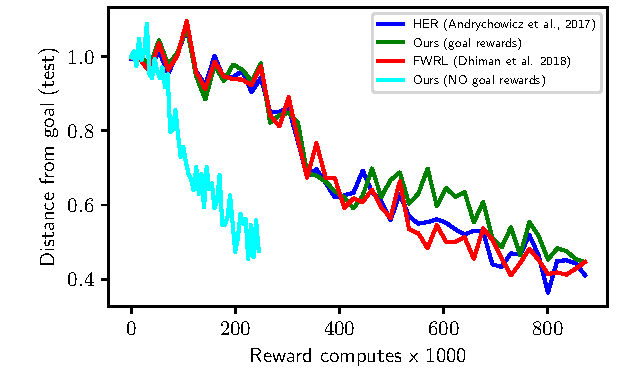
\includegraphics[width=\frac\columnwidth]{media/res/6efc1de-path_reward_low_thresh_chosen-HandManipulateEggFullPR-v0-dqst/reward_computes-test/ag_g_dist.pdf}%
  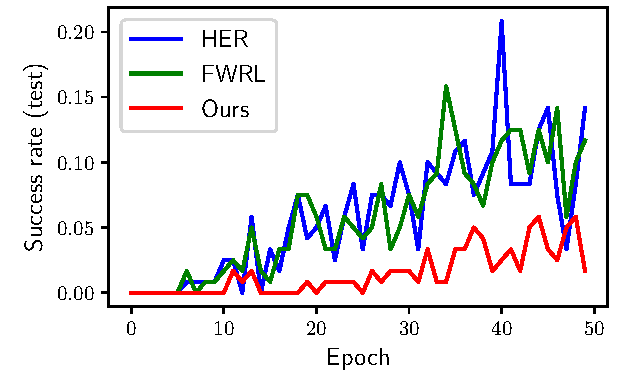
\includegraphics[width=\frac\columnwidth]{media/res/6efc1de-path_reward_low_thresh_chosen-HandManipulateEggFullPR-v0-dqst/epoch-test/success_rate.pdf}%
  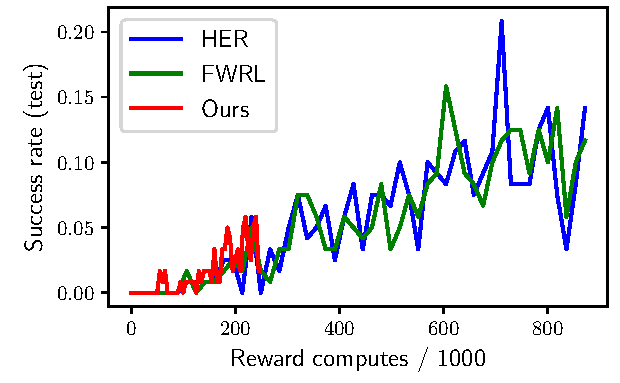
\includegraphics[width=\frac\columnwidth]{media/res/6efc1de-path_reward_low_thresh_chosen-HandManipulateEggFullPR-v0-dqst/reward_computes-test/success_rate.pdf}\\
  \rotatebox{90}{{\tiny \hspace{0.5cm} \color{blue}{Hand Pen Rotate}}}%
  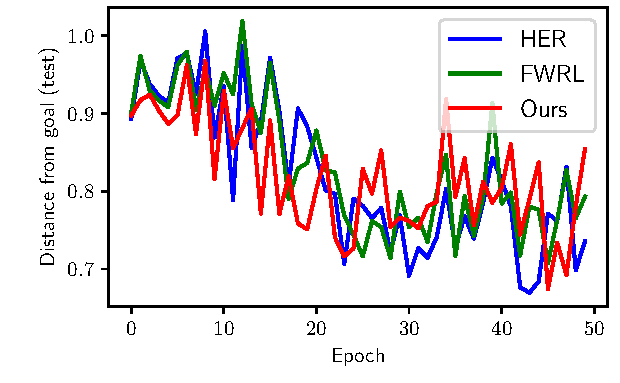
\includegraphics[width=\frac\columnwidth]{media/res/6efc1de-path_reward_low_thresh_chosen-HandManipulatePenRotate-v0-ddpg/epoch-test/ag_g_dist.pdf}%
  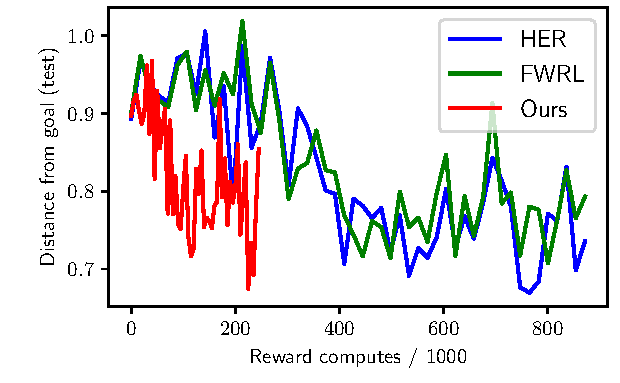
\includegraphics[width=\frac\columnwidth]{media/res/6efc1de-path_reward_low_thresh_chosen-HandManipulatePenRotate-v0-ddpg/reward_computes-test/ag_g_dist.pdf}%
  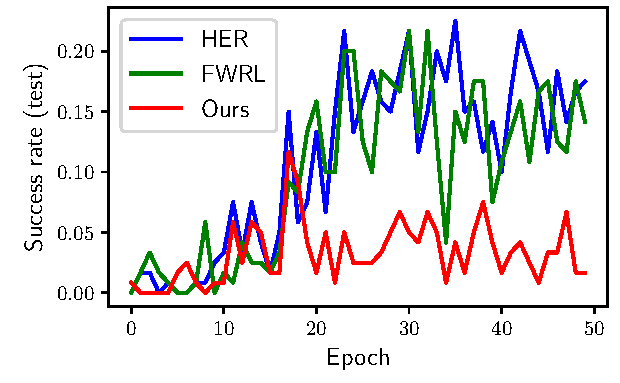
\includegraphics[width=\frac\columnwidth]{media/res/6efc1de-path_reward_low_thresh_chosen-HandManipulatePenRotate-v0-ddpg/epoch-test/success_rate.pdf}%
  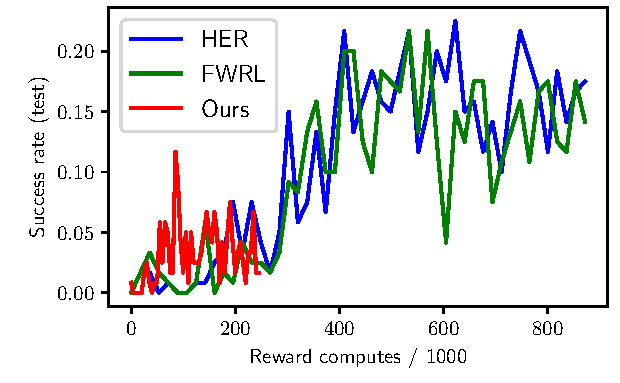
\includegraphics[width=\frac\columnwidth]{media/res/6efc1de-path_reward_low_thresh_chosen-HandManipulatePenRotate-v0-ddpg/reward_computes-test/success_rate.pdf}
  {.\tiny\color{blue}\hspace{0.8cm}(a) Distance on Epochs \hspace{1.05cm}(b) Distance on
    reward computes
    \hspace{0.70cm} (c) Success rate on epochs \hspace{0.9cm} (d) Success rate on reward computes}
  \caption{For the hand tasks, we compare our method (red) against HER (blue) ~\citep{andrychowicz2016learning}
    and FWRL (green) ~\citep{dhiman2018floydwarshall} for the distance-from-goal
    and success rate metrics. Furthermore, both metrics are plotted
    against two progress measures, the number of training epochs and the number of reward
    computations. Measured by distance from the goal, our method performs comparable to or
    better than the baselines for both progress measurements. For the success rate,
    our method underperforms against the baselines. 
}%
  \label{fig:hand-results}%
\end{figure}%
% 

